\documentclass[14pt]{extarticle}
% =============================================================================
% Shared Preamble for Worksheets, Homeworks, Exams & Lesson Notes
% (scripts/tex_preamble.tex)
% =============================================================================

\newif\ifdetailed
\ifdefined\setdetailed
  \setdetailed
\fi

\newif\ifwithsols
\ifdefined\setwithsols
  \setwithsols
\fi

\newif\ifwhiteblack
\ifdefined\setwhiteblack
  \setwhiteblack
\fi

% Document-class specific packages (loaded before common_preamble.tex / polyglossia)
\usepackage{fancyhdr}
\usepackage{enumitem}
\usepackage{titlesec}
\usepackage[bottom]{footmisc}
\usepackage{titling}
\usepackage{longtable} % page-breakable tables
\usepackage{float}
\usepackage[onehalfspacing]{setspace}

\ifwhiteblack
  \usepackage[a4paper, landscape, top=1.25cm, bottom=1.25cm, left=1.25cm, right=1.25cm, headheight=1.5cm, headsep=0.5cm]{geometry}
\else
  \usepackage[a4paper, top=2.4cm, bottom=2.4cm, left=2.2cm, right=2.2cm, headheight=1.4cm, headsep=0.4cm, footskip=1.0cm]{geometry}
\fi

% Shared common packages, fonts, polyglossia, callout boxes, code helpers, date & header macros
\IfFileExists{scripts/common_preamble.tex}{%
  % =============================================================================
% Shared Common Preamble (scripts/common_preamble.tex)
% Included by:
%   - scripts/tex_preamble.tex    (worksheets, homeworks, exams, lesson notes)
%   - scripts/book_preamble.tex   (two-sided Arabic book)
%   - scripts/beamer_preamble.tex (Beamer presentation slides)
% =============================================================================

\usepackage{fontspec}
\usepackage{amsmath}
\usepackage{amssymb}
\usepackage{xcolor}
\usepackage{graphicx}
\usepackage{listings}
\usepackage[most]{tcolorbox}
\usepackage{pifont}
\usepackage{minted}
\usepackage{etoolbox}
\usepackage{array}
\usepackage{booktabs}
\usepackage{tikz}
\usepackage{datetime2}

\usetikzlibrary{automata, positioning, arrows.meta, arrows, shapes.geometric, calc}

% Beamer already loads hyperref internally; load it here for article/book classes
% right before polyglossia (bidi).
\makeatletter
\@ifclassloaded{beamer}{}{%
  \usepackage{hyperref}%
  \hypersetup{hidelinks}%
  \providecommand{\LTcaptype}{table}%
}
\makeatother

% Load polyglossia (and bidi) AFTER graphics, tables, boxes, code, and hyperref
\usepackage{polyglossia}
\setmainlanguage[numerals=western]{arabic}
\setotherlanguage{english}
\newfontfamily\arabicfont[Script=Arabic]{Calibri}
\newfontfamily\arabicfontsf[Script=Arabic]{Calibri}
\newfontfamily\arabicfonttt[Script=Arabic]{Courier New}
\newfontfamily\emoji[BoldFont=*,ItalicFont=*]{Segoe UI Emoji}

% Allow slight inter-word stretch to avoid Overfull \hbox with inline \textenglish
\emergencystretch=1.5em

% -----------------------------------------------------------------------------
% Default Minted & Callout Box Definitions
% -----------------------------------------------------------------------------
\AtBeginEnvironment{minted}{\setstretch{0.95}}
\setminted{fontsize=\small, breaklines=true, vspace=2pt}

\tcbset{
  arc=2.5pt, outer arc=2.5pt,
  boxsep=1pt, left=6pt, right=6pt, top=3pt, bottom=3pt,
  toptitle=1.5pt, bottomtitle=1.5pt,
  before skip=6pt, after skip=6pt,
  fonttitle=\bfseries,
  fontupper=\setstretch{1.1}\setlength{\parskip}{2pt},
  colback=white, colframe=black, boxrule=0.6pt,
  boxcolor/.style 2 args={colback=#1, colframe=#2}
}

\newtcolorbox{boxDef}[1][]{boxcolor={blue!4!white}{blue!75!black},
  title={{\emoji📘} تعريف\ifx\\#1\\\else ~#1\fi :}}
\newtcolorbox{boxExercise}[1][]{boxcolor={cyan!4!white}{cyan!70!black},
  title={{\emoji🧩} تمرين\ifx\\#1\\\else ~#1\fi :}}
\newtcolorbox{boxExample}[1][]{boxcolor={yellow!6!white}{orange!85!black},
  title={{\emoji📝} مثال\ifx\\#1\\\else ~#1\fi :}}
\newtcolorbox{boxNote}[1][]{boxcolor={gray!7!white}{black!75},
  title={{\emoji✨} ملاحظة\ifx\\#1\\\else ~#1\fi :}}
\newtcolorbox{boxAttention}[1][]{boxcolor={magenta!5!white}{magenta!75!black},
  title={{\emoji🔔} تنبيه\ifx\\#1\\\else ~#1\fi :}}
\newtcolorbox{boxWarning}[1][]{boxcolor={red!4!white}{red!75!black},
  title={{\emoji⚡} ملاحظة هامة\ifx\\#1\\\else ~#1\fi :}}
\newtcolorbox{boxSolution}[1][]{boxcolor={green!4!white}{green!60!black},
  title={{\emoji✅} حل\ifx\\#1\\\else ~#1\fi :}}
\newtcolorbox{boxSymbol}[1][]{boxcolor={purple!4!white}{purple!70!black},
  title={{\emoji🔣} رمز\ifx\\#1\\\else ~#1\fi :}}
\newtcolorbox{boxHint}[1][]{boxcolor={teal!4!white}{teal!65!black},
  title={{\emoji💡} تلميح\ifx\\#1\\\else ~#1\fi :}}

% Compact code boxes: tighter line spacing and small vertical gaps
\tcbset{
  simplecode/.style={
    arc=2pt, outer arc=2pt,
    left=4pt, right=4pt, top=4pt, bottom=4pt,
    fontupper=\setstretch{0.95},
    before skip=6pt, after skip=6pt,
    colback=gray!5, colframe=black!50, boxrule=0.4pt
  }
}
\newenvironment{boxCode}{\begin{tcolorbox}[simplecode]}{\end{tcolorbox}}

% Code cell used inside tables (keeps code left-to-right inside RTL tables)
% Use inside a fixed-width p{...} column: \begin{pycell}\begin{minted}...\end{minted}\end{pycell}
\makeatletter
\newtcolorbox{pycell}{frame empty,colback=white,boxsep=0pt,left=2pt,right=2pt,top=2pt,bottom=2pt,width=\linewidth,before=\noindent,after=,baseline={\tcb@height-\ht\strutbox},fontupper=\setstretch{0.95}\setlength{\topsep}{0pt}\setlength{\partopsep}{0pt}\setlength{\parskip}{0pt}}
\makeatother

\newcolumntype{C}[1]{>{\centering\arraybackslash}p{#1}}

% Dotted date style (DD.MM.YYYY)
\makeatletter
\DTMnewdatestyle{dotted}{%
  \renewcommand{\DTMdisplaydate}[4]{\two@digits{##3}.\two@digits{##2}.##1}%
  \renewcommand{\DTMDisplaydate}{\DTMdisplaydate}%
}
\makeatother
\DTMsetdatestyle{dotted}

% -----------------------------------------------------------------------------
% Customizable Header / Footer Metadata
% -----------------------------------------------------------------------------
\newcommand{\headerleft}{مدرسة التسامح الشاملة}
\newcommand{\headerright}{الأستاذ محمود اغبارية}
\newcommand{\footercenter}{\thepage}

\newcommand{\setheaderleft}[1]{\renewcommand{\headerleft}{#1}}
\newcommand{\setheaderright}[1]{\renewcommand{\headerright}{#1}}
\newcommand{\setfootercenter}[1]{\renewcommand{\footercenter}{#1}}
%
}{%
  \IfFileExists{../../../scripts/common_preamble.tex}{%
    % =============================================================================
% Shared Common Preamble (scripts/common_preamble.tex)
% Included by:
%   - scripts/tex_preamble.tex    (worksheets, homeworks, exams, lesson notes)
%   - scripts/book_preamble.tex   (two-sided Arabic book)
%   - scripts/beamer_preamble.tex (Beamer presentation slides)
% =============================================================================

\usepackage{fontspec}
\usepackage{amsmath}
\usepackage{amssymb}
\usepackage{xcolor}
\usepackage{graphicx}
\usepackage{listings}
\usepackage[most]{tcolorbox}
\usepackage{pifont}
\usepackage{minted}
\usepackage{etoolbox}
\usepackage{array}
\usepackage{booktabs}
\usepackage{tikz}
\usepackage{datetime2}

\usetikzlibrary{automata, positioning, arrows.meta, arrows, shapes.geometric, calc}

% Beamer already loads hyperref internally; load it here for article/book classes
% right before polyglossia (bidi).
\makeatletter
\@ifclassloaded{beamer}{}{%
  \usepackage{hyperref}%
  \hypersetup{hidelinks}%
  \providecommand{\LTcaptype}{table}%
}
\makeatother

% Load polyglossia (and bidi) AFTER graphics, tables, boxes, code, and hyperref
\usepackage{polyglossia}
\setmainlanguage[numerals=western]{arabic}
\setotherlanguage{english}
\newfontfamily\arabicfont[Script=Arabic]{Calibri}
\newfontfamily\arabicfontsf[Script=Arabic]{Calibri}
\newfontfamily\arabicfonttt[Script=Arabic]{Courier New}
\newfontfamily\emoji[BoldFont=*,ItalicFont=*]{Segoe UI Emoji}

% Allow slight inter-word stretch to avoid Overfull \hbox with inline \textenglish
\emergencystretch=1.5em

% -----------------------------------------------------------------------------
% Default Minted & Callout Box Definitions
% -----------------------------------------------------------------------------
\AtBeginEnvironment{minted}{\setstretch{0.95}}
\setminted{fontsize=\small, breaklines=true, vspace=2pt}

\tcbset{
  arc=2.5pt, outer arc=2.5pt,
  boxsep=1pt, left=6pt, right=6pt, top=3pt, bottom=3pt,
  toptitle=1.5pt, bottomtitle=1.5pt,
  before skip=6pt, after skip=6pt,
  fonttitle=\bfseries,
  fontupper=\setstretch{1.1}\setlength{\parskip}{2pt},
  colback=white, colframe=black, boxrule=0.6pt,
  boxcolor/.style 2 args={colback=#1, colframe=#2}
}

\newtcolorbox{boxDef}[1][]{boxcolor={blue!4!white}{blue!75!black},
  title={{\emoji📘} تعريف\ifx\\#1\\\else ~#1\fi :}}
\newtcolorbox{boxExercise}[1][]{boxcolor={cyan!4!white}{cyan!70!black},
  title={{\emoji🧩} تمرين\ifx\\#1\\\else ~#1\fi :}}
\newtcolorbox{boxExample}[1][]{boxcolor={yellow!6!white}{orange!85!black},
  title={{\emoji📝} مثال\ifx\\#1\\\else ~#1\fi :}}
\newtcolorbox{boxNote}[1][]{boxcolor={gray!7!white}{black!75},
  title={{\emoji✨} ملاحظة\ifx\\#1\\\else ~#1\fi :}}
\newtcolorbox{boxAttention}[1][]{boxcolor={magenta!5!white}{magenta!75!black},
  title={{\emoji🔔} تنبيه\ifx\\#1\\\else ~#1\fi :}}
\newtcolorbox{boxWarning}[1][]{boxcolor={red!4!white}{red!75!black},
  title={{\emoji⚡} ملاحظة هامة\ifx\\#1\\\else ~#1\fi :}}
\newtcolorbox{boxSolution}[1][]{boxcolor={green!4!white}{green!60!black},
  title={{\emoji✅} حل\ifx\\#1\\\else ~#1\fi :}}
\newtcolorbox{boxSymbol}[1][]{boxcolor={purple!4!white}{purple!70!black},
  title={{\emoji🔣} رمز\ifx\\#1\\\else ~#1\fi :}}
\newtcolorbox{boxHint}[1][]{boxcolor={teal!4!white}{teal!65!black},
  title={{\emoji💡} تلميح\ifx\\#1\\\else ~#1\fi :}}

% Compact code boxes: tighter line spacing and small vertical gaps
\tcbset{
  simplecode/.style={
    arc=2pt, outer arc=2pt,
    left=4pt, right=4pt, top=4pt, bottom=4pt,
    fontupper=\setstretch{0.95},
    before skip=6pt, after skip=6pt,
    colback=gray!5, colframe=black!50, boxrule=0.4pt
  }
}
\newenvironment{boxCode}{\begin{tcolorbox}[simplecode]}{\end{tcolorbox}}

% Code cell used inside tables (keeps code left-to-right inside RTL tables)
% Use inside a fixed-width p{...} column: \begin{pycell}\begin{minted}...\end{minted}\end{pycell}
\makeatletter
\newtcolorbox{pycell}{frame empty,colback=white,boxsep=0pt,left=2pt,right=2pt,top=2pt,bottom=2pt,width=\linewidth,before=\noindent,after=,baseline={\tcb@height-\ht\strutbox},fontupper=\setstretch{0.95}\setlength{\topsep}{0pt}\setlength{\partopsep}{0pt}\setlength{\parskip}{0pt}}
\makeatother

\newcolumntype{C}[1]{>{\centering\arraybackslash}p{#1}}

% Dotted date style (DD.MM.YYYY)
\makeatletter
\DTMnewdatestyle{dotted}{%
  \renewcommand{\DTMdisplaydate}[4]{\two@digits{##3}.\two@digits{##2}.##1}%
  \renewcommand{\DTMDisplaydate}{\DTMdisplaydate}%
}
\makeatother
\DTMsetdatestyle{dotted}

% -----------------------------------------------------------------------------
% Customizable Header / Footer Metadata
% -----------------------------------------------------------------------------
\newcommand{\headerleft}{مدرسة التسامح الشاملة}
\newcommand{\headerright}{الأستاذ محمود اغبارية}
\newcommand{\footercenter}{\thepage}

\newcommand{\setheaderleft}[1]{\renewcommand{\headerleft}{#1}}
\newcommand{\setheaderright}[1]{\renewcommand{\headerright}{#1}}
\newcommand{\setfootercenter}[1]{\renewcommand{\footercenter}{#1}}
%
  }{%
    \input{../../scripts/common_preamble.tex}%
  }%
}

\pagestyle{fancy}

% Prevent widow/orphan lines
\widowpenalty=10000
\clubpenalty=10000

% Compact section headings and default list spacing so pages do not waste vertical space
\titlespacing*{\section}{0pt}{1.4ex plus 0.4ex minus 0.2ex}{0.7ex plus 0.2ex}
\titlespacing*{\subsection}{0pt}{1.1ex plus 0.3ex minus 0.2ex}{0.5ex plus 0.1ex}
\titlespacing*{\subsubsection}{0pt}{0.9ex plus 0.2ex minus 0.1ex}{0.4ex plus 0.1ex}
\setlist{topsep=4pt, partopsep=0pt, parsep=2pt, itemsep=4pt}

\gappto\captionsarabic{\renewcommand{\contentsname}{جدول المحتويات}}

% Legacy listings settings
\lstset{
  language=[Sharp]C,
  numbers=left,
  stepnumber=1,
  numbersep=8pt,
  frame=single,
  basicstyle=\ttfamily\small
}
\ifwhiteblack
  \lstset{
    keywordstyle=\bfseries,
    stringstyle=\ttfamily,
    commentstyle=\itshape
  }
\else
  \lstset{
    keywordstyle=\color{blue},
    stringstyle=\color{red},
    commentstyle=\color{green!50!black}
  }
\fi

% White-and-black landscape presentation mode overrides
\ifwhiteblack
  \AtBeginDocument{
    \LARGE
    \usemintedstyle{bw}
  }
  \setminted{vspace=2pt}
  \tcbset{
    colback=white, colframe=black, boxrule=1pt,
    boxcolor/.style 2 args={colback=white, colframe=black},
    simplecode/.append style={colback=white, colframe=black, boxrule=1pt}
  }
\fi

% Default to empty author to avoid "LaTeX Warning: No \author given" when omitted
\author{}

% Compact title block
\makeatletter
\renewcommand{\@maketitle}{%
  \begin{center}%
    {\ifwhiteblack\Huge\else\LARGE\fi \bfseries \@title \par}%
    \ifdefempty{\@author}{}{%
      \vskip 0.15em%
      {\large \@author \par}%
    }%
    {\small \hfill \textenglish{\DTMtoday} \par}%
  \end{center}%
  \vspace{-0.3cm}%
}
\makeatother

\apptocmd{\maketitle}{\thispagestyle{fancy}}{}{}

% Apply page headers and footer (using \headerleft, \headerright, \footercenter from common_preamble.tex)
\newcommand{\applyfancyheaders}{%
  \fancyhf{}%
  \fancyhead[L]{\textarabic{\headerleft}}%
  \fancyhead[R]{\textarabic{\headerright}}%
  \fancyfoot[C]{\textarabic{\footercenter}}%
}

\fancypagestyle{plain}{\applyfancyheaders}
\applyfancyheaders

\setcounter{tocdepth}{3} % only section, subsection, and subsubsection in TOC

\newcommand{\importpdfpage}[2]{%
    \newgeometry{left=0cm,right=0cm,top=0cm,bottom=0cm}
    \thispagestyle{empty}
    \includegraphics[page=#2,width=0.95\paperwidth,height=0.95\paperheight,keepaspectratio]{#1}
    \restoregeometry
}

\newcommand{\insertFullImg}[1]{%
    \noindent
    \makebox[\textwidth][c]{
        \includegraphics[width=0.9\paperwidth,keepaspectratio]{#1}%
    }%
}%


\usetikzlibrary{arrows.meta, positioning, shapes.geometric, fit, backgrounds}

\title{الملخّص الشامل للبرمجة الموجّهة كائنات في \textenglish{C\#} --- دليل البجروت}

\begin{document}

\maketitle
\thispagestyle{fancy}

\begin{boxDef}[- هدف هذا الملخّص]
يجمع هذا الدليل بصورةٍ واضحة ومباشرة جميع مفاهيم البرمجة الموجّهة كائنات وأفكار امتحانات البجروت في لغة \textenglish{C\#}، وفق الترتيب نفسه المُعتمد في الحصص الصفّية: الفئات والمؤشّرات والصفات الساكنة، التوريث والاحتواء والعمليات البنائية، تعدّد الأشكال وتحديد العملية المُستدعاة والأخطاء الشائعة، والفئات المجرّدة وواجهات التطبيق. صيغ الشرح بعربيةٍ سلسةٍ وواضحةٍ مدعومةٍ بالأمثلة والرسوم التوضيحية.
\end{boxDef}

% ==============================================================
\section*{الجزء الأوّل: الفئات، المؤشّرات، والصفات الساكنة}
% ==============================================================

\subsection*{$1$. الفئة، التغليف (\textenglish{Get}/\textenglish{Set})، العمليات البنائية، و\textenglish{ToString()}}
\textbf{الفكرة:} الفئة هي قالبٌ نُنشئ منه كائنات في الذاكرة؛ ولكلّ كائنٍ نسختُه الخاصّة من الصفات. نُعرّف الصفات بإذن وصول \textenglish{private} لحمايتها من التعديل العشوائي، ونتيح قراءتها عبر \textenglish{Get} وتعديلها بأمان عبر \textenglish{Set} أو عملياتٍ تفحص صحّة المُعطيات \textbf{قبل} تغيير حالة الكائن.

العملية البنائية تُستدعى تلقائيًا لحظة إنشاء الكائن بـ \textenglish{new} لتهيئة صفاته؛ وهي تحمل اسم الفئة نفسه بلا نمط إرجاع (حتى \textenglish{void} لا تُكتب)، ويمكن استدعاء عملية بنائية أخرى في الفئة نفسها عبر \textenglish{: this(...)} لمنع التكرار. أمّا العملية \textenglish{ToString()} فنُعيد تعريفها بـ \textenglish{override} لتُعيد نصًّا يصف الكائن تلقائيًا عند طباعته بـ \textenglish{Console.WriteLine}.

\begin{boxCode}
\begin{english}
\begin{minted}{csharp}
public class BankAccount
{
    private string owner;
    private double balance;
    public BankAccount(string owner, double balance)
    {
        this.owner = owner;
        if (balance >= 0) { this.balance = balance; }
        else { this.balance = 0; }
    }
    public BankAccount(string owner) : this(owner, 0) { }
    public bool Withdraw(double amount)
    {
        if (amount <= 0 || amount > this.balance) { return false; }
        this.balance -= amount;
        return true;
    }
    public override string ToString()
    {
        return $"Owner:{this.owner}, Balance:{this.balance}";
    }
}
// In Main:
BankAccount acc = new BankAccount("Lina", 500);
acc.Withdraw(120);
Console.WriteLine(acc); // Automatically calls acc.ToString()
\end{minted}
\end{english}
\end{boxCode}

\textbf{تنبيه:} بمجرّد كتابة أيّ عملية بنائية في الفئة، تُلغى العملية البنائية الافتراضية الفارغة تلقائيًا؛ فإن احتجناها وجبت كتابتها صراحةً. كما أنّ \textenglish{ToString()} \textbf{تُعيد} نصًّا ولا تطبع داخله.

\filbreak
\subsection*{$2$. المؤشّرات في الذاكرة، المرجعية المشتركة، والعملية البنائية الناسخة}
\textbf{الفكرة:} المتغيّر من نمط فئة لا يحمل الكائن نفسه، بل يحفظ \textbf{مؤشّرًا} (عنوانًا) يدلّ على مكان الكائن في الذاكرة. لذلك، عندما نكتب \textenglish{s2 = s1} فإنّنا ننسخ المؤشّر فقط، فيشير المتغيّران إلى \textbf{نفس الكائن} (مرجعية مشتركة)، وأيّ تعديلٍ عبر أحدهما يظهر في الآخر. أمّا إذا أردنا كائنًا مستقلًّا يحمل القيم نفسها، فنستخدم \textbf{عملية بنائية ناسخة} (\textenglish{new Sensor(s1)})، وكذلك نُنشئ نسخةً دفاعيةً لحماية كائنٍ مُحتوى داخل فئة أخرى.

\begin{boxCode}
\begin{english}
\begin{minted}{csharp}
public class Sensor
{
    private int temp;
    public Sensor(int temp) { this.temp = temp; }
    public Sensor(Sensor other) { this.temp = other.temp; } // Copy ctor
    public int GetTemp() { return this.temp; }
    public void SetTemp(int t) { this.temp = t; }
}
public class Room
{
    private Sensor s;
    public Room(Sensor s) { this.s = new Sensor(s); } // Defensive copy!
    public Sensor GetSensor() { return new Sensor(this.s); }
}
// Case A (Reference copy): Sensor s1 = new Sensor(22); Sensor s2 = s1; s2.SetTemp(40);
// Case B (Deep copy):      Sensor s1 = new Sensor(22); Sensor s2 = new Sensor(s1); s2.SetTemp(40);
\end{minted}
\end{english}
\end{boxCode}

\begin{center}
\begin{english}
\begin{tikzpicture}[
    var/.style={rectangle, draw=blue!70!black, fill=blue!8, thick, minimum width=1.2cm, minimum height=0.6cm, font=\small},
    obj/.style={rectangle, rounded corners=4pt, draw=teal!75!black, fill=teal!8, thick, minimum width=2.5cm, minimum height=0.8cm, align=center, font=\footnotesize},
    arr/.style={-{Stealth[length=2.6mm]}, thick, draw=blue!75!black}
]
    \node[font=\small\bfseries, text=red!70!black, align=center] (t1) {\textarabic{الحالة \textenglish{A}: نسخ المؤشّر}\\[-1pt]\scriptsize\texttt{s2 = s1; s2.SetTemp(40);}};
    \node[var, below left=0.35cm and 0.2cm of t1] (p1) {\texttt{s1}};
    \node[var, below=0.45cm of p1] (p2) {\texttt{s2}};
    \node[obj, draw=red!70!black, fill=red!6, right=1.1cm of p1, yshift=-0.52cm] (o1) {\texttt{Sensor}\\\texttt{temp = }\textbf{40}};
    \draw[arr] (p1.east) -- (o1.west);
    \draw[arr] (p2.east) -- (o1.west);

    \node[font=\small\bfseries, text=teal!75!black, align=center, right=3.4cm of t1] (t2) {\textarabic{الحالة \textenglish{B}: نسخ عميق}\\[-1pt]\scriptsize\texttt{s2 = new Sensor(s1); s2.SetTemp(40);}};
    \node[var, below left=0.35cm and 0.2cm of t2] (q1) {\texttt{s1}};
    \node[var, below=0.55cm of q1] (q2) {\texttt{s2}};
    \node[obj, right=1.1cm of q1] (o2) {\texttt{Sensor}\\\texttt{temp = 22}};
    \node[obj, right=1.1cm of q2] (o3) {\texttt{Sensor}\\\texttt{temp = }\textbf{40}};
    \draw[arr] (q1.east) -- (o2.west);
    \draw[arr] (q2.east) -- (o3.west);
\end{tikzpicture}
\end{english}
\end{center}

\textbf{تنبيه:} المقارنة \textenglish{s1 == s2} تفحص تساوي \textbf{المؤشّرين} لا تساوي القيم. كما أنّ إنشاء مصفوفة \textenglish{new Sensor[5]} يُنشئ $5$ مؤشّراتٍ قيمتها \textenglish{null} لا $5$ كائنات.

\filbreak
\subsection*{$3$. الصفات والعمليات الساكنة والثوابت (\textenglish{static} و \textenglish{const}) في الوراثة}
\textbf{الفكرة:} الصفة العادية تتكرّر لكلّ كائنٍ على حدة، أمّا الصفة المعرّفة بـ \textenglish{static} فتُوجد منها \textbf{نسخة واحدة فقط مشتركة} بين جميع كائنات الفئة وجميع كائنات الفئات الوارثة منها؛ ولذلك تُستعمل في البجروت كثيرًا كعدّادٍ للكائنات المُنشأة. أمّا \textenglish{const} فيُعرّف قيمةً ثابتةً لا تتغيّر، والعملية الساكنة تُستدعى عبر اسم الفئة مباشرةً (\textenglish{Device.GetTotal()}).

\begin{boxCode}
\begin{english}
\begin{minted}{csharp}
public class Device
{
    public const int WARRANTY_YEARS = 2;
    protected static int totalDevices = 0; // Shared by Device & subclasses
    private int id;
    public Device()
    {
        totalDevices++;
        this.id = totalDevices;
    }
    public static int GetTotal() { return totalDevices; } // No 'this' here
}
public class Phone : Device
{
    public Phone() : base() { }
}
// In Main:
Device d1 = new Device(); // totalDevices = 1, d1.id = 1
Phone p1  = new Phone();  // Calls base() -> totalDevices = 2, p1.id = 2
Console.WriteLine(Device.GetTotal()); // Prints: 2
\end{minted}
\end{english}
\end{boxCode}

\textbf{تنبيه:} داخل عملية \textenglish{static} لا يمكن استعمال \textenglish{this} ولا الوصول إلى الصفات غير الساكنة.

% ==============================================================
\clearpage
\section*{الجزء الثاني: التوريث، مخطّط الفئات، والعمليات البنائية}
% ==============================================================

\subsection*{$4$. تصميم الهرمية: التوريث مقابل الاحتواء ومخطّط الفئات}
\textbf{الفكرة:} عند تصميم منظومةٍ مُحَوسَبةٍ نُميّز بدقّة بين علاقتين أساسيتين:
\begin{itemize}
    \item \textbf{التوريث (علاقة «هو نوع من»):} عندما تشترك عدّة فئاتٍ في صفاتٍ وعملياتٍ متطابقة، نجمع المشترك في فئة أبٍ واحدة وترثه الفئات الابنة عبر \textenglish{class StudentMember : Member}. يُرمز له بسهم \textbf{مثلّث فارغ} يتّجه من الابن إلى الأب.
    \item \textbf{الاحتواء / التركيب (علاقة «يحتوي على»):} عندما تحفظ فئةٌ داخلها كائنًا أو مصفوفة كائناتٍ من فئة أخرى كصفة (مثل عضوٍ يمتلك خطّة دفع \textenglish{Plan}). يُرمز له بسهم \textbf{معيّن ممتلئ} عند الفئة الحاوية.
\end{itemize}

\begin{center}
\begin{english}
\begin{tikzpicture}[
    cls/.style={rectangle, rounded corners=3pt, draw=black!80, fill=gray!6, thick, text width=3.3cm, align=center, inner sep=5pt, font=\footnotesize},
    inh/.style={-{Triangle[open, length=3.2mm, width=2.8mm]}, thick, draw=blue!75!black},
    comp/.style={{Diamond[length=3.4mm, width=2.4mm]}-, thick, draw=teal!80!black}
]
    \node[cls] (M) {\textbf{\texttt{Member}}\\[-1pt]\scriptsize\texttt{\# string id}\\\scriptsize\texttt{\# Plan plan}};
    \node[cls, right=2.2cm of M] (P) {\textbf{\texttt{Plan}}\\[-1pt]\scriptsize\texttt{- double monthlyFee}\\\scriptsize\texttt{- int months}};
    \node[cls, below left=1.0cm and -0.4cm of M] (S) {\textbf{\texttt{StudentMember}}\\[-1pt]\scriptsize\texttt{- double discount}};
    \node[cls, below right=1.0cm and -0.4cm of M] (V) {\textbf{\texttt{VipMember}}\\[-1pt]\scriptsize\texttt{- int extraBooks}};

    \draw[comp] (M.east) -- node[above, font=\scriptsize, text=teal!80!black]{\textarabic{احتواء}} (P.west);
    \draw[inh] (S.north) -- node[left, xshift=-2pt, font=\scriptsize, text=blue!75!black]{\textarabic{توريث}} (M.south west);
    \draw[inh] (V.north) -- node[right, xshift=2pt, font=\scriptsize, text=blue!75!black]{\textarabic{توريث}} (M.south east);
\end{tikzpicture}
\end{english}
\end{center}

\begin{boxCode}
\begin{english}
\begin{minted}{csharp}
public class Plan { private double monthlyFee; private int months; }
public class Member
{
    protected string id;
    protected Plan plan; // Composition (has-a)
}
public class StudentMember : Member { private double discount; }
public class VipMember : Member     { private int extraBooks; }
\end{minted}
\end{english}
\end{boxCode}

\filbreak
\subsection*{$5$. أذونات الوصول (\textenglish{private}، \textenglish{protected}، \textenglish{public}) وتظليل الصفات}
\textbf{الفكرة:} ترث الفئة الابنة جميع صفات الأب (فهي موجودةٌ فعليًا داخل كائن الابن في الذاكرة)، لكنّها \textbf{لا تستطيع الوصول مباشرةً} إلى الصفات المعرّفة كـ \textenglish{private} في الأب، بل تتعامل معها عبر عمليات \textenglish{Get}/\textenglish{Set}. أمّا إذن الوصول \textenglish{protected} فيُبقي الصفة محميةً عن الخارج مع إتاحتها مباشرةً للأبناء.

{\renewcommand{\arraystretch}{1.15}
\small
\begin{longtable}{|C{0.20\textwidth}|C{0.10\textwidth}|C{0.18\textwidth}|C{0.18\textwidth}|C{0.18\textwidth}|}
\hline
\textbf{إذن الوصول} & \textbf{الرمز} & \textbf{داخل الفئة} & \textbf{الفئة الوارثة} & \textbf{خارج الفئة} \\
\hline
\textenglish{private} & $-$ & نعم & لا & لا \\
\hline
\textenglish{protected} & $\#$ & نعم & نعم & لا \\
\hline
\textenglish{public} & $+$ & نعم & نعم & نعم \\
\hline
\end{longtable}}

\begin{boxCode}
\begin{english}
\begin{minted}{csharp}
public class Box
{
    private int x;
    public Box(int x) { this.x = x; }
    public int GetParentX() { return this.x; }
}
public class SpecialBox : Box
{
    private int x; // SHADOWING: separate field from Box.x!
    public SpecialBox(int a, int b) : base(a) { this.x = b; }
    public int GetChildX() { return this.x; }
}
// SpecialBox sb = new SpecialBox(10, 99);
// sb.GetParentX() -> 10,  sb.GetChildX() -> 99
\end{minted}
\end{english}
\end{boxCode}

\textbf{تنبيه (تظليل الصفات):} لا تُعد كتابة صفة موروثة من الأب داخل الابن؛ لأنّ ذلك يُنشئ \textbf{صفتين منفصلتين} داخل الكائن نفسه.

\filbreak
\subsection*{$6$. العمليات البنائية في الوراثة (\textenglish{: base(...)}) وتسلسل التنفيذ}
\textbf{الفكرة:} \textbf{العمليات البنائية لا تُورَّث.} عند إنشاء كائنٍ من فئةٍ ابنةٍ يبدأ التنفيذ دائمًا من \textbf{أعلى الهرمية نزولًا إلى الابن}: يُنفَّذ جسم العملية البنائية للأب أوّلًا ثم جسم الابن. نُمرّر المعطيات إلى الأب عبر \textenglish{: base(...)}، وإذا لم نكتبها فإنّ \textenglish{C\#} تضيف \textenglish{: base()} تلقائيًا.

\begin{boxCode}
\begin{english}
\begin{minted}{csharp}
public class A { public A() { Console.WriteLine("A"); } }
public class B : A { public B() : base() { Console.WriteLine("B"); } }
public class C : B { public C() : base() { Console.WriteLine("C"); } }
// C obj = new C();  --> Output: A, then B, then C
\end{minted}
\end{english}
\end{boxCode}

\begin{center}
\begin{english}
\begin{tikzpicture}[
    cstep/.style={rectangle, rounded corners=4pt, draw=blue!70!black, fill=blue!7, thick, minimum width=2.9cm, minimum height=0.8cm, align=center, font=\footnotesize},
    arr/.style={-{Stealth[length=2.6mm]}, thick}
]
    \node[cstep] (c1) {\texttt{new C()}\\\scriptsize\textarabic{يستدعي \textenglish{base()}}};
    \node[cstep, right=1.1cm of c1] (b1) {\texttt{B()}\\\scriptsize\textarabic{يستدعي \textenglish{base()}}};
    \node[cstep, right=1.1cm of b1, draw=teal!75!black, fill=teal!10] (a1) {\texttt{A()}\\\scriptsize\textarabic{يطبع \textenglish{"A"} أوّلًا}};
    \node[cstep, below=0.7cm of b1, draw=teal!75!black, fill=teal!10] (b2) {\textarabic{يطبع \textenglish{"B"} ثانيًا}};
    \node[cstep, below=0.7cm of c1, draw=teal!75!black, fill=teal!10] (c2) {\textarabic{يطبع \textenglish{"C"} أخيرًا}};

    \draw[arr, blue!75!black] (c1.east) -- (b1.west);
    \draw[arr, blue!75!black] (b1.east) -- (a1.west);
    \draw[arr, teal!80!black] (a1.south) |- (b2.east);
    \draw[arr, teal!80!black] (b2.west) -- (c2.east);
\end{tikzpicture}
\end{english}
\end{center}

ومثالٌ على العمليات البنائية الافتراضية وبالمعطيات والناسخة في الوراثة:

\begin{boxCode}
\begin{english}
\begin{minted}{csharp}
public class Parent
{
    protected int a;
    public Parent()             { this.a = 5; }
    public Parent(int a)        { this.a = a; }
    public Parent(Parent other) { this.a = other.a + 1; }
}
public class Child : Parent
{
    private int b;
    public Child(int x) : base(x * 2) { this.b = this.a + 3; }
    public Child(Parent p) : base(p)  { this.b = 10; }
}
// Parent p1 = new Parent(4); -> a = 4
// Child  c1 = new Child(3);  -> base(6) -> a = 6, b = 9
// Child  c2 = new Child(p1); -> base(p1) calls Copy ctor -> a = 5, b = 10
\end{minted}
\end{english}
\end{boxCode}

\textbf{تنبيه:} إذا لم تكن في الأب عملية بنائية افتراضية بلا معطيات، وكتبنا بنائيةً في الابن دون \textenglish{: base(...)} صريحة $\leftarrow$ ينتج \textbf{خطأ في التجميع}.

% ==============================================================
\clearpage
\section*{الجزء الثالث: تعدّد الأشكال، تحديد العملية المُستدعاة، والتحويل، والأخطاء}
% ==============================================================

\subsection*{$7$. التحويل لأعلى، المصفوفة متعدّدة الأشكال، والفئة \textenglish{Object}}
\textbf{الفكرة:} متغيّر من نمط الأب (أو من نمط \textenglish{Object} الذي ترث منه جميع الفئات تلقائيًا) يستطيع الإشارة إلى كائنٍ من أيّ فئةٍ ابنةٍ ترث منه؛ هذا هو \textbf{التحويل لأعلى} وهو سليمٌ دائمًا. وبفضله نجمع كائناتٍ من أنماطٍ فرعيةٍ مختلفة في مصفوفة واحدة (\textenglish{Media[]} أو \textenglish{Object[]}). ولإرجاع مصفوفةٍ مُصفّاةٍ بحجمٍ دقيق نمسح المصفوفة \textbf{مرّتين}: الأولى للعدّ وبناء المصفوفة، والثانية لنسخ المؤشّرات باستخدام مؤشّر مستقلّ $k$.

\begin{boxCode}
\begin{english}
\begin{minted}{csharp}
public static Media[] GetLongItems(Media[] arr, int minMinutes)
{
    int count = 0;
    for (int i = 0; i < arr.Length; i++)
    {
        if (arr[i] != null && arr[i].GetDuration() >= minMinutes) { count++; }
    }
    Media[] res = new Media[count];
    int k = 0;
    for (int i = 0; i < arr.Length; i++)
    {
        if (arr[i] != null && arr[i].GetDuration() >= minMinutes)
        {
            res[k] = arr[i];
            k++;
        }
    }
    return res;
}
\end{minted}
\end{english}
\end{boxCode}

\textbf{تنبيه:} افحص دائمًا \textenglish{arr[i] != null} ولا تتوقّف بـ \textenglish{break} عند أوّل حدٍّ فارغ.

\filbreak
\subsection*{$8$. إعادة تعريف العمليات (\textenglish{virtual}، \textenglish{override}، و\textenglish{base})}
\textbf{الفكرة:} عندما تشترك الفئات الوارثة في سلوكٍ واحدٍ يختلف حسابه من فئةٍ لأخرى، نعرّف العملية في الأب بـ \textenglish{virtual} ونعيد تعريفها في الأبناء بـ \textenglish{override} بالتعريف نفسه تمامًا. وعند استدعائها عبر مؤشّر الأب تُنفّذ نسخة الكائن الفعلي تلقائيًا (دون الحاجة إلى \textenglish{is} أو \textenglish{as}). ويمكن للابن الاستفادة من حساب الأب عبر \textenglish{base.GetCost()} أو \textenglish{base.ToString()}.

\begin{boxCode}
\begin{english}
\begin{minted}{csharp}
public class Delivery
{
    protected double km;
    public Delivery(double km) { this.km = km; }
    public virtual double GetCost() { return 20 + this.km * 2.5; }
}
public class ExpressDelivery : Delivery
{
    public ExpressDelivery(double km) : base(km) { }
    public override double GetCost() { return base.GetCost() + 35; }
}
public class DroneDelivery : Delivery
{
    public DroneDelivery(double km) : base(km) { }
    public override double GetCost() { return base.GetCost() * 0.8; }
}
\end{minted}
\end{english}
\end{boxCode}

\textbf{تنبيه:} نسيان \textenglish{base.} داخل \textenglish{override} (كتابة \textenglish{return GetCost() + 35;}) يؤدّي إلى استدعاءٍ تراجعيٍّ لا نهائيّ (\textenglish{StackOverflowException})!

\filbreak
\subsection*{$9$. القاعدة الذهبية لتحديد العملية المُستدعاة (زمن التجميع مقابل زمن التشغيل)}
\textbf{الفكرة:} عند استدعاء عملية مثل \textenglish{x.Calc(y)} يمرّ الحاسوب بـ\textbf{خطوتين منفصلتين تمامًا}:
\begin{enumerate}[itemsep=0.35em]
    \item \textbf{في زمن التجميع (مسح الأوامر):} ينظر المُجمّع \textbf{فقط إلى النمط الساكن} لكلٍّ من المتغيّر $x$ والمُعطى $y$، ويختار أنسب توقيعٍ مطابق (وإن لم يجد $\leftarrow$ \textbf{خطأ في التجميع}).
    \item \textbf{في زمن التشغيل (تنفيذ الأوامر):} إذا كانت العملية المختارة في الخطوة ($1$) تحمل \textenglish{virtual} أو \textenglish{override} أو \textenglish{abstract} $\leftarrow$ ينزل إلى \textbf{آخر \textenglish{override}} لها في النمط الفعلي للكائن $x$؛ وإلّا ينفّذ نفس العملية المختارة في الخطوة ($1$) مباشرةً.
\end{enumerate}

\begin{center}
\begin{english}
\begin{tikzpicture}[
    box/.style={rectangle, rounded corners=5pt, draw=blue!65!black, fill=blue!6, thick, text width=5.9cm, align=center, inner sep=5pt, font=\footnotesize},
    runbox/.style={rectangle, rounded corners=5pt, draw=teal!70!black, fill=teal!7, thick, text width=5.4cm, align=center, inner sep=5pt, font=\footnotesize},
    errbox/.style={rectangle, rounded corners=5pt, draw=red!70!black, fill=red!7, thick, text width=3.8cm, align=center, inner sep=5pt, font=\footnotesize},
    dec/.style={rectangle, rounded corners=4pt, draw=orange!80!black, fill=orange!10, thick, text width=5.5cm, align=center, inner sep=5pt, font=\footnotesize},
    arr/.style={-{Stealth[length=2.6mm]}, thick, draw=black!75}
]
    \node[box] (step1) {\textbf{\textarabic{الخطوة $1$: زمن التجميع}}\\[1pt]
        \textarabic{فحص النمط الساكن للمتغيّر وللمُعطيات واختيار التوقيع الأنسب}};
    \node[errbox, right=1.1cm of step1] (err) {\textbf{\textarabic{خطأ في التجميع}}\\[1pt]
        \textarabic{لا توجد عملية مطابقة}};
    \node[dec, below=0.7cm of step1] (check) {\textbf{\textarabic{الخطوة $2$: زمن التشغيل}}\\[1pt]
        \textarabic{هل العملية المختارة \textenglish{virtual} / \textenglish{override}؟}};
    \node[runbox, below left=0.75cm and -1.6cm of check] (yes) {\textbf{\textarabic{نعم (ربط ديناميكي)}}\\[1pt]
        \textarabic{استدعاء آخر \textenglish{override} في النمط الفعلي}};
    \node[runbox, draw=purple!70!black, fill=purple!6, below right=0.75cm and -1.6cm of check] (no) {\textbf{\textarabic{لا (ربط ساكن)}}\\[1pt]
        \textarabic{تنفيذ نفس العملية المختارة في الخطوة $1$}};

    \draw[arr] (step1.east) -- node[above, font=\scriptsize]{\textarabic{لا توجد}} (err.west);
    \draw[arr] (step1.south) -- node[right, font=\scriptsize]{\textarabic{وُجِدت}} (check.north);
    \draw[arr] (check.west) -| node[pos=0.25, above, font=\scriptsize]{\textarabic{نعم}} (yes.north);
    \draw[arr] (check.east) -| node[pos=0.25, above, font=\scriptsize]{\textarabic{لا}} (no.north);
\end{tikzpicture}
\end{english}
\end{center}

\filbreak
\textbf{لماذا نحتاج \textenglish{virtual} و\textenglish{override}؟} لاحظ الفارق عند \textenglish{P c = new Q(); c.Print();}:
\begin{boxCode}
\begin{english}
\begin{minted}{csharp}
// Case 1 (WITHOUT virtual/override): c.Print() stops at P -> prints "P"
// Case 2 (WITH virtual/override):    c.Print() goes to Q  -> prints "Q"
\end{minted}
\end{english}
\end{boxCode}

\begin{center}
\begin{english}
\begin{tikzpicture}[
    var/.style={rectangle, draw=blue!70!black, fill=blue!8, thick, minimum width=2.2cm, minimum height=0.85cm, align=center},
    partA/.style={rectangle, draw=black!75, fill=gray!10, thick, minimum width=3.8cm, minimum height=0.82cm, align=center, font=\small},
    partB/.style={rectangle, draw=teal!75!black, fill=teal!10, thick, minimum width=3.8cm, minimum height=0.82cm, align=center, font=\small},
    arr/.style={-{Stealth[length=2.6mm]}, thick}
]
    \node[var] (c) {\texttt{P c}\\[-1pt]\scriptsize\textarabic{النمط الساكن: \textenglish{P}}};
    \node[partA, right=1.0cm of c, yshift=0.41cm] (objA) {\texttt{P.Print()} $\rightarrow$ \texttt{"P"}};
    \node[partB, below=0pt of objA] (objB) {\texttt{Q.Print()} $\rightarrow$ \texttt{"Q"}};
    \begin{scope}[on background layer]
        \node[draw=teal!80!black, dashed, rounded corners=4pt, fit=(objA)(objB), inner sep=4pt,
              label={[teal!80!black, font=\scriptsize]above:{\textarabic{الكائن الفعلي: \textenglish{\texttt{new Q()}}}}}] (heap) {};
    \end{scope}
    \draw[arr, blue!75!black] (c.east) -- node[above, font=\scriptsize]{\textarabic{مؤشّر}} (heap.west);
    \node[right=0.85cm of objA, align=right, font=\footnotesize, text=purple!80!black] (lbl1)
        {\textarabic{الحالة $1$ (بدون \textenglish{virtual}): يتوقّف هنا $\leftarrow$ \textenglish{"P"}}};
    \node[right=0.85cm of objB, align=right, font=\footnotesize, text=teal!80!black] (lbl2)
        {\textarabic{الحالة $2$ (مع \textenglish{virtual}/\textenglish{override}): ينزل هنا $\leftarrow$ \textenglish{"Q"}}};
    \draw[arr, purple!80!black] (objA.east) -- (lbl1.west);
    \draw[arr, teal!80!black, dashed] (objA.south east) to[bend right=35] (objB.north east);
    \draw[arr, teal!80!black] (objB.east) -- (lbl2.west);
\end{tikzpicture}
\end{english}
\end{center}

\filbreak
\textbf{مثال شامل على نمط البجروت (دمج التحميل الزائد مع \textenglish{virtual} و\textenglish{override}):}
\begin{boxCode}
\begin{english}
\begin{minted}{csharp}
public class P
{
    public virtual void Calc(Q x) { Console.WriteLine("P.Calc(Q)"); }
}
public class Q : P
{
    public override void Calc(Q x) { Console.WriteLine("Q.Calc(Q)"); }
    public void Calc(P x)          { Console.WriteLine("Q.Calc(P)"); }
}
public class R : Q
{
    public override void Calc(Q x) { Console.WriteLine("R.Calc(Q)"); }
    public void Calc(R x)          { Console.WriteLine("R.Calc(R)"); }
}
// In Main:
P pq = new Q();   // Static: P, Runtime: Q
P pr = new R();   // Static: P, Runtime: R
Q qr = new R();   // Static: Q, Runtime: R
R r  = new R();   // Static: R, Runtime: R
\end{minted}
\end{english}
\end{boxCode}

\begin{center}
\begin{english}
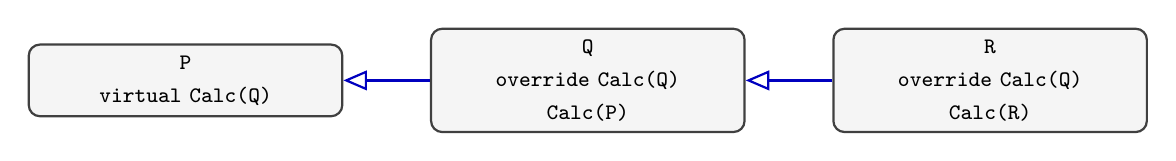
\begin{tikzpicture}[
    cls/.style={rectangle, rounded corners=4pt, draw=black!75, fill=gray!8, thick, text width=3.7cm, align=center, inner sep=4pt, font=\footnotesize},
    inh/.style={-{Triangle[open, length=3mm, width=2.5mm]}, thick, draw=blue!75!black}
]
    \node[cls] (P) {\textbf{\texttt{P}}\\\texttt{virtual Calc(Q)}};
    \node[cls, right=1.1cm of P] (Q) {\textbf{\texttt{Q}}\\\texttt{override Calc(Q)}\\\texttt{Calc(P)}};
    \node[cls, right=1.1cm of Q] (R) {\textbf{\texttt{R}}\\\texttt{override Calc(Q)}\\\texttt{Calc(R)}};
    \draw[inh] (Q.west) -- (P.east);
    \draw[inh] (R.west) -- (Q.east);
\end{tikzpicture}
\end{english}
\end{center}

{\renewcommand{\arraystretch}{1.2}
\small
\begin{longtable}{|>{\raggedright\arraybackslash}p{0.21\textwidth}|>{\raggedleft\arraybackslash}p{0.26\textwidth}|>{\raggedleft\arraybackslash}p{0.25\textwidth}|>{\raggedright\arraybackslash}p{0.15\textwidth}|}
\hline
\textbf{أمر الاستدعاء} & \textbf{الخطوة $1$: زمن التجميع} & \textbf{الخطوة $2$: زمن التشغيل} & \textbf{المُخرَج} \\
\hline
\endfirsthead
\hline
\textbf{أمر الاستدعاء} & \textbf{الخطوة $1$: زمن التجميع} & \textbf{الخطوة $2$: زمن التشغيل} & \textbf{المُخرَج} \\
\hline
\endhead
\textenglish{pr.Calc(qr);} &
الساكن $P$ والمُعطى $Q$ $\leftarrow$ \textenglish{P.Calc(Q)} (\textenglish{virtual}). &
الفعلي $R$ $\leftarrow$ آخر \textenglish{override} في $R$. &
\textenglish{R.Calc(Q)} \\
\hline
\textenglish{r.Calc(pr);} &
الساكن $R$ والمُعطى $P$ $\leftarrow$ \textenglish{Q.Calc(P)} الموروثة (ليست \textenglish{virtual}). &
ليست \textenglish{virtual} $\leftarrow$ تُنفّذ مباشرةً. &
\textenglish{Q.Calc(P)} \\
\hline
\textenglish{((Q)pq).Calc(pq);} &
الساكن بعد التحويل $Q$ والمُعطى $P$ $\leftarrow$ \textenglish{Q.Calc(P)}. &
التحويل سليم (الفعلي $Q$) $\leftarrow$ تُنفّذ مباشرةً. &
\textenglish{Q.Calc(P)} \\
\hline
\textenglish{pq.Calc(pr);} &
في $P$ توجد فقط \textenglish{Calc(Q)}، والمُعطى ساكنه $P$! &
لا يصل لزمن التشغيل. &
\textarabic{\textbf{خطأ تجميع}} \\
\hline
\end{longtable}}

\begin{boxWarning}[- الفخّ الأكثر تكرارًا في البجروت]
في السطر \textenglish{r.Calc(pr);} لا تنخدع لأنّ الكائن الفعلي لـ \textenglish{pr} هو $R$! تذكّر دائمًا: النمط الفعلي يؤثّر فقط على \textbf{الكائن الذي قبل النقطة} (إذا كانت العملية \textenglish{virtual} أو \textenglish{override})؛ أمّا \textbf{المُعطى داخل الأقواس فيُحسَم دائمًا حسب نمطه الساكن في زمن التجميع!}
\end{boxWarning}

\filbreak
\subsection*{$10$. التحويل لأسفل وفحص النمط (\textenglish{is} و \textenglish{as}) والعمليات الخارجية}
\textbf{الفكرة:} لتفعيل عمليةٍ خاصّةٍ بالابن عبر متغيّرٍ نمطه الساكن أب، نحتاج إلى \textbf{تحويلٍ لأسفل}. لتفادي انهيار البرنامج نفحص النمط أوّلًا بـ \textenglish{is} ثم نحوّل بـ \textenglish{(Parrot)x}، أو نستخدم \textenglish{x as Parrot} التي تعيد \textenglish{null} عند عدم التوافق.

\begin{boxCode}
\begin{english}
\begin{minted}{csharp}
// Suppose Parrot : Bird : Animal, Bird has Fly(), Parrot has Talk()
public static void ShowAbilities(Animal[] arr)
{
    for (int i = 0; i < arr.Length; i++)
    {
        if (arr[i] is Parrot)    { ((Parrot)arr[i]).Talk(); } // Specific FIRST!
        else if (arr[i] is Bird) { ((Bird)arr[i]).Fly(); }
    }
}
\end{minted}
\end{english}
\end{boxCode}

{\renewcommand{\arraystretch}{1.15}
\small
\begin{longtable}{|C{0.22\textwidth}|C{0.18\textwidth}|C{0.28\textwidth}|C{0.16\textwidth}|}
\hline
\textbf{الأسلوب} & \textbf{عند التوافق} & \textbf{عند عدم التوافق} & \textbf{مع \textenglish{null}} \\
\hline
\textenglish{is} ثم \textenglish{(Bird)x} & ينجح & يمنع التحويل بأمان & \textenglish{false} \\
\hline
\textenglish{x as Bird} & ينجح & يعيد \textenglish{null} & \textenglish{null} \\
\hline
\textenglish{(Bird)x} مباشرةً & ينجح & \textbf{خطأ زمن تشغيل} (\textenglish{InvalidCastException}) & \textenglish{null} \\
\hline
\end{longtable}}

\textbf{تنبيه:} انتبه لأمرَين: (1) فحص \textbf{الفئة الأخصّ أوّلًا} في \textenglish{if / else if} لأنّ كلّ \textenglish{Parrot} هو أيضًا \textenglish{Bird}، (2) وضع الأقواس حول التحويل قبل النقطة: \textenglish{((Bird)arr[i]).Fly()}.

\filbreak
\subsection*{$11$. دليل التمييز بين خطأ التجميع وخطأ زمن التشغيل}
سؤال \textbf{«هل قطعة الكود سليمة أم غير سليمة؟ وحدّد نوع الخطأ»} من أكثر أسئلة البجروت تكرارًا. افترض أنّ \textenglish{Y} فيها \textenglish{virtual void F1()}، و\textenglish{Z : Y} فيها \textenglish{override void F1()} و\textenglish{void F2()}، ولدينا \textenglish{Y a = new Y(); Y b = new Z();}:

{\renewcommand{\arraystretch}{1.18}
\small
\begin{longtable}{|>{\raggedright\arraybackslash}p{0.28\textwidth}|C{0.20\textwidth}|>{\raggedleft\arraybackslash}p{0.38\textwidth}|}
\hline
\textbf{قطعة الكود} & \textbf{الحكم} & \textbf{التفسير} \\
\hline
\endfirsthead
\hline
\textbf{قطعة الكود} & \textbf{الحكم} & \textbf{التفسير} \\
\hline
\endhead
\textenglish{Z z = new Y();} & \textbf{خطأ تجميع} & لا يجوز تعيين أب في متغيّر ابن بدون تحويل. \\
\hline
\textenglish{Z z = (Z)a;} & \textbf{خطأ زمن تشغيل} & الصياغة سليمة، لكن الكائن الفعلي \textenglish{Y} ليس \textenglish{Z}. \\
\hline
\textenglish{b.F2();} & \textbf{خطأ تجميع} & النمط الساكن لـ \textenglish{b} هو \textenglish{Y} ولا يعرف \textenglish{F2()}. \\
\hline
\textenglish{((Z)b).F2();} & \textbf{سليم} & التحويل سليم (الفعلي \textenglish{Z}) فتُستدعى \textenglish{Z.F2()}. \\
\hline
\textenglish{Object o = b; ((Y)o).F1();} & \textbf{سليم} & الفعلي \textenglish{Z} هو أيضًا \textenglish{Y}، وتُنفّذ \textenglish{Z.F1()}. \\
\hline
\end{longtable}}

\filbreak
\subsection*{$12$. رسم الكائنات والمؤشّرات في الذاكرة (مخطّط الكائنات)}
\textbf{الفكرة:} في أسئلة البجروت الحديثة يُطلب عرض الكائنات التي تكوّنت في الذاكرة مع ذكر \textbf{النمط الفعلي للكائن، والنمط الساكن للمؤشّر (نوع التوجيه)، وقيم جميع الصفات} (الموروثة والخاصّة). انتبه خاصةً عندما يشير حدّان في المصفوفة إلى نفس الكائن!

\begin{boxCode}
\begin{english}
\begin{minted}{csharp}
A[] arr = new A[3];
arr[0] = new B(5); // Static: A, Runtime: B (fields of A + B)
arr[1] = arr[0];   // Points to the SAME B object as arr[0]!
arr[2] = new A(1); // Static: A, Runtime: A (fields of A only)
\end{minted}
\end{english}
\end{boxCode}

\filbreak
\subsection*{$13$. إعادة تعريف العملية \textenglish{Equals} ومقارنة الكائنات}
\textbf{الفكرة:} جميع الفئات ترث من \textenglish{Object} العملية \textenglish{Equals(object obj)} التي تقارن المؤشّرين افتراضيًا. لمقارنة قيم الصفات نعيد تعريفها بـ \textenglish{override} بثلاث خطواتٍ ثابتة: فحص \textenglish{null} ونمط الكائن بـ \textenglish{is}، ثم التحويل، ثم مقارنة الصفات.

\begin{boxCode}
\begin{english}
\begin{minted}{csharp}
public class Product
{
    private string code;
    public override bool Equals(object obj)
    {
        if (obj == null || !(obj is Product)) { return false; }
        Product other = (Product)obj;
        return this.code.Equals(other.code);
    }
}
\end{minted}
\end{english}
\end{boxCode}

\textbf{تنبيه:} كتابة \textenglish{public bool Equals(Product other)} هي \textbf{تحميل زائد} وليست إعادة تعريف!

% ==============================================================
\clearpage
\section*{الجزء الرابع: الفئات المجرّدة، واجهات التطبيق، والدمج الشامل}
% ==============================================================

\subsection*{$14$. الفئة المجرّدة والعمليات المجرّدة (\textenglish{abstract}) والمُعطى العام \textenglish{object}}
\textbf{الفكرة:} الفئة المجرّدة هي فئة أساسية لا يُسمح بإنشاء كائنٍ مباشرٍ منها (\textenglish{new Notification()} خطأ تجميع)، لكن يجوز تعريف متغيّراتٍ ومصفوفاتٍ من نمطها (\textenglish{new Notification[5]} سليم!). العملية المجرّدة تُكتب بتعريفها فقط وتنتهي بـ \textenglish{;}، وتُلزم كلّ ابنٍ غير مجرّد بتطبيقها بـ \textenglish{override}. وعندما تختلف أنماط المُعطيات بين الأبناء، نوحّد التعريف بمُعطى من نمط \textenglish{object} ونفحصه بـ \textenglish{is}.

\begin{boxCode}
\begin{english}
\begin{minted}{csharp}
public abstract class Notification
{
    protected string target;
    public Notification(string target) { this.target = target; }
    public abstract bool Send(object payload);
}
public class SmsNotif : Notification
{
    public SmsNotif(string phone) : base(phone) { }
    public override bool Send(object payload)
    {
        if (payload is string)
        {
            Console.WriteLine("SMS to " + this.target + ": " + (string)payload);
            return true;
        }
        return false;
    }
}
\end{minted}
\end{english}
\end{boxCode}

\textbf{تنبيه:} عند تمرير عددٍ صحيحٍ مثل $20$ داخل \textenglish{object o}، فإنّ \textenglish{o is double} يعيد \textenglish{false} لأنّ القيمة المغلّفة هي \textenglish{int} لا \textenglish{double}.

\filbreak
\subsection*{$15$. واجهات التطبيق (\textenglish{interface}) وقواعد الترتيب والدمج مع التوريث}
\textbf{الفكرة:} واجهة التطبيق هي عَقْد برمجيّ يحدّد عناوين عملياتٍ فقط (بلا صفاتٍ ولا عملياتٍ بنائية)، وتلتزم كلّ فئةٍ تطبّقها بكتابة أجسامها بإذن وصول \textenglish{public} (دون \textenglish{override}). ترث الفئة من \textbf{فئة أبٍ واحدة فقط}، لكنها تستطيع تطبيق \textbf{عدّة واجهات تطبيق معًا}.

\begin{boxCode}
\begin{english}
\begin{minted}{csharp}
public interface ITaxable   { double GetTax(); }
public interface IPrintable { void PrintReport(); }
public class Asset          { protected double value; }

// CORRECT: base class Asset FIRST, then interfaces!
public class Apartment : Asset, ITaxable, IPrintable
{
    public double GetTax()    { return this.value * 0.02; } // No 'override'!
    public void PrintReport() { Console.WriteLine("Tax: " + this.GetTax()); }
}
// WRONG (Compile Error): public class Apartment : ITaxable, Asset { ... }
\end{minted}
\end{english}
\end{boxCode}

\begin{boxWarning}[- قاعدة الترتيب الإلزامية في \textenglish{C\#}]
عند دمج التوريث مع واجهات التطبيق، \textbf{يجب كتابة الفئة الأب أوّلًا} ثم أسماء الواجهات؛ وعكس الترتيب يسبّب \textbf{خطأ في التجميع}. كما يُمنع إنشاء كائنٍ من واجهةٍ بـ \textenglish{new ITaxable()}.
\end{boxWarning}

\filbreak
\subsection*{$16$. الواجهة \textenglish{IComparable}، الفرز العام، والدمج الشامل}
\textbf{الفكرة:} الواجهة \textenglish{IComparable} تُلزم الفئة بتطبيق \textenglish{int CompareTo(object obj)} التي تعيد \textbf{عددًا سالبًا} إذا كان \textenglish{this} أصغر، و\textbf{صفرًا} عند التساوي، و\textbf{عددًا موجبًا} إذا كان أكبر؛ ممّا يتيح فرز أيّ مصفوفة \textenglish{IComparable[]} بعملية فرزٍ عامّةٍ واحدة، وكذلك تصفية كائناتٍ من نمطٍ معيّن بـ \textenglish{is} ثم فرزها دون تغيير المصفوفة الأصلية.

\begin{boxCode}
\begin{english}
\begin{minted}{csharp}
public class Course : IComparable
{
    private double credits;
    public int CompareTo(object obj)
    {
        if (obj == null || !(obj is Course)) { return 1; }
        Course other = (Course)obj;
        if (this.credits < other.credits) { return -1; } // Safe for double!
        if (this.credits > other.credits) { return 1; }
        return 0;
    }
}
public static void SortAscending(IComparable[] arr)
{
    for (int i = 0; i < arr.Length - 1; i++)
    {
        for (int j = 0; j < arr.Length - 1 - i; j++)
        {
            if (arr[j].CompareTo(arr[j + 1]) > 0)
            {
                IComparable tmp = arr[j];
                arr[j] = arr[j + 1];
                arr[j + 1] = tmp;
            }
        }
    }
}
\end{minted}
\end{english}
\end{boxCode}

\textbf{تنبيه:} مع الأعداد العشرية (\textenglish{double}) لا تكتب \textenglish{(int)(this.credits - other.credits)} لأنّ الفرق $0.5$ يتحوّل إلى $0$!

\filbreak
{\renewcommand{\arraystretch}{1.15}
\small
\begin{longtable}{|C{0.24\textwidth}|C{0.20\textwidth}|C{0.20\textwidth}|C{0.22\textwidth}|}
\hline
\textbf{وجه المقارنة} & \textbf{فئة عادية} & \textbf{فئة مجرّدة} & \textbf{واجهة تطبيق} \\
\hline
إنشاء كائن بـ \textenglish{new} & مسموح & ممنوع & ممنوع \\
\hline
صفات وعمليات بنائية & نعم & نعم & لا \\
\hline
عمليات مطبّقة (بجسم) & نعم & نعم (مع مجرّدة) & لا (عناوين فقط) \\
\hline
عدد ما يمكن وراثته/تطبيقه & أب واحد فقط & أب واحد فقط & عدّة واجهات معًا \\
\hline
\end{longtable}}

\filbreak
\begin{boxAttention}[- قائمة مراجعة سريعة قبل تسليم حلّ البجروت]
\begin{enumerate}[itemsep=0.2em]
    \item هل استعملتُ \textenglish{protected} للصفات التي يحتاجها الأبناء، و\textenglish{: base(...)} في العمليات البنائية؟
    \item هل استعنتُ بـ \textenglish{base.ToString()} أو \textenglish{base.Method()} لتجنّب تكرار كود الأب؟
    \item هل فحصتُ \textenglish{!= null} و\textenglish{is} (بالترتيب من الأخصّ إلى الأعمّ) قبل أيّ تحويلٍ لأسفل؟
    \item عند تتبّع استدعاء عملية: هل فصلتُ بين \textbf{زمن التجميع} (النمط الساكن للمتغيّر والمُعطى) و\textbf{زمن التشغيل} (آخر \textenglish{override} في النمط الفعلي)؟
    \item عند دمج التوريث مع واجهة تطبيق: هل كتبتُ الفئة الأب أوّلًا قبل أسماء الواجهات؟
\end{enumerate}
\end{boxAttention}

\vspace{0.8cm}
\begin{flushleft}
أرجو لكم وقتًا ممتعًا.

الأستاذ محمود اغبارية.
\end{flushleft}

\end{document}
